\section{How Does Memory Work?}

\subsection{Key Terms}
%TODO extract into a glossary
\begin{itemize}
  \item \textbf{Capacitors} - Stores electrical energy by accumulating electric charge. Two terminals, one in and one out.
  \item \textbf{Transistor} - Amplifies or switches electrical signals. Uses three terminals, a current or voltage applied to one terminal (normally the middle terminal) will control the conductance of the semiconducting material from the first terminal to the last terminal. See figure~\ref{fig-tran}.
\end{itemize}

\begin{figure}
\centering
  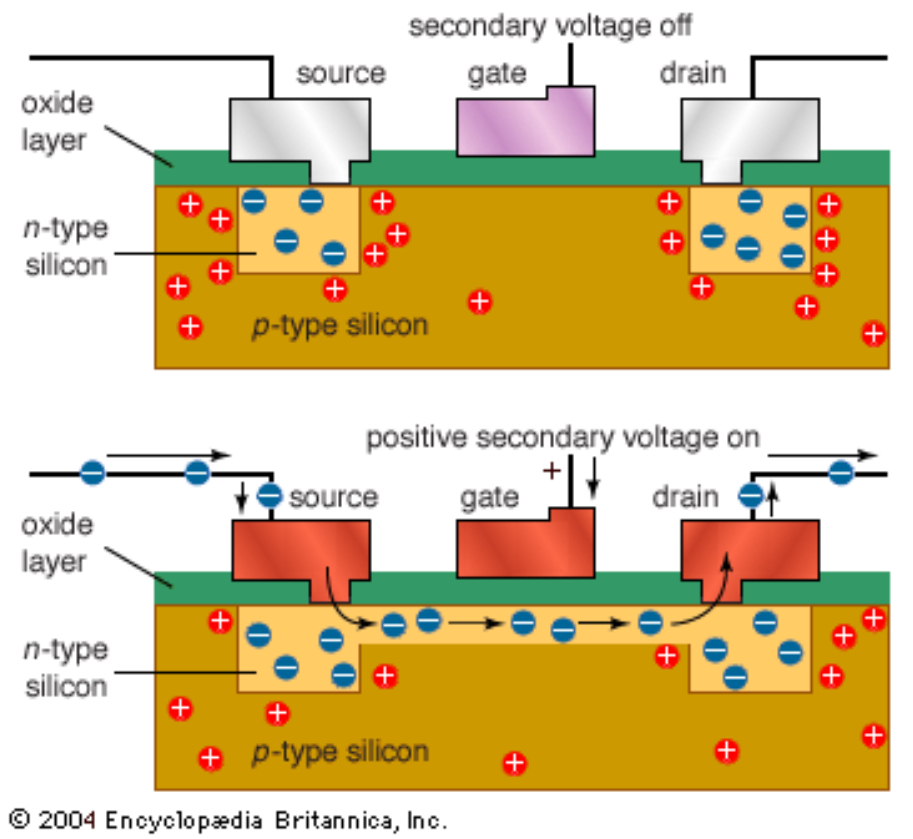
\includegraphics[scale=0.25]{./chapters/hardware-background/assets/pnp.png}
  \caption{An NPN Transistor~\cite{britannica-transistor}}\label{fig-tran}
\end{figure}
